\documentclass[letterpaper, 9pt, conference]{ieeeconf}

\usepackage{amssymb}\usepackage{amsmath}\usepackage{amsfonts}
\usepackage[mathcal, mathscr]{eucal}
\usepackage{graphicx}
%\usepackage{epstopdf}
\newcommand{\vect}{\boldsymbol}
\newcommand{\matr}{\boldsymbol}
\newcommand{\diag}{\textrm{diag}}
\usepackage{algorithm}
\usepackage{algorithmic}

\IEEEoverridecommandlockouts       % This command is only
                                                          % needed if you want to
                                                          % use the \thanks command
\overrideIEEEmargins
% See the \addtolength command later in the file to balance the column lengths
% on the last page of the document



% The following packages can be found on http:\\www.ctan.org
%\usepackage{graphics} % for pdf, bitmapped graphics files
%\usepackage{epsfig} % for postscript graphics files
%\usepackage{mathptmx} % assumes new font selection scheme installed
%\usepackage{times} % assumes new font selection scheme installed
%\usepackage{amsmath} % assumes amsmath package installed
%\usepackage{amssymb}  % assumes amsmath package installed

\title{\LARGE \bf
Recurrence network analysis of multiple band oscillations of local field potentials from the primary motor cortex reveals rich dynamics.
}


% PIN:  26810 (ZC),
% 42117 (KT), 17447 (NGH)

\author{Narayan Puthanmadam Subramaniyam, {\em Student Member, IEEE}, Jari Hyttinen, {\em Senior Member, IEEE}, \\
Jos\'{e} Iriarte-D\'{i}az, Nicholas G. Hatsopoulos, Callum F. Ross, and 
Kazutaka Takahashi, {\em Senior Member, IEEE} \\
\thanks{N.P. Subramaniyam and J. Hyttine are with Department of Elecronics and Communications Engineering, Tampere University o Technology. 
(Email: \{narayan.ps, jari.hyttinen\}@tut.fi.) This work is financially supported by International Doctoral Programme in Biomedical Engineering and Medical Physics (iBioMEP) – Academy of Finland, Decision No. 141171. K. Takahashi is with Department of Organismal Biology and Anatomy, University of Chicago, IL 60637 USA. 
 (Email: kazutaka@uchicago.edu). This work was supported by NIH R01.}}

\begin{document}



\maketitle
\thispagestyle{empty}
\pagestyle{empty}



\begin{abstract}
Aggregate signals that reflect activities of a large number of neurons in the cerebral cortex, local field potentials (LFPs) have been observed to mediate gross functional activities of a relatively small volume of the brain tissues. There are several bands of the oscillations frequencies in LFPs that have been observed across multiple brain areas. 
The signature oscillation band of the LFPs in the primary motor cortex (MI) is over $\beta$ range and it has been consistently observed both in human and non-human primates around the time of visual cues and movement onsets. 
However, its dynamical behavior has not been well characterized. Furthermore, dynamics of $\beta$ oscillations has been documented based on the phase locking of $\beta$ oscillations, but not in terms of the inherent dynamics of the oscillations themselves. Here, we used the complexity measure derived from cluster coefficients of a recurrence network and analyzed a pair of wide-band signals, one including $\beta$ band of the LFPs and the other ranging the low $\gamma$ band  in MI recorded from a non-human primate. We show rather unique temporal profiles of the evoked responses using complexity of the dynamical behavior in both bands of the oscillation, either of which is not simply resembling either the power of the oscillation or the phase locking of $\beta$ oscillations. Therefore, the current method can reveal a new type
of dynamics of the underlying network complexity during the task simply simply based on event evoked potentials of wide-band oscillatory signals. 
\end{abstract}

\begin{keywords}
Local field potentials, event evoked potentials, recurrence network, temporal dynamics, motor cortex, functional connectivity
\end{keywords}



\section{Introduction}
Cortical rhythms have been extensively studied since early descriptions of oscillations in sensorimotor cortex by Jasper and Penfield \cite{jasper1949}. Since In particular, local field potentials (LFPs) and electroencephalograms (EEG) in the $\beta$ frequency range (15-30 Hz) are ubiquitous in the motor cortex of mammals including monkeys and humans across the upper limb area of the primary motor cortex (MI). The dynamics of the $\beta$ oscillation has been grossly characterized, based on a temporal profile of the amplitude of the oscillations, such as event related synchronization (ERS) and event related desynchronization (ERD) \cite{neuper2001, Jurkiewicz20061281}, and phase locking to the instruction cues \cite{jake2011}. However, the dynamical properties of $\beta$ oscillations have not been well characterized. Recently, it has been reported that phase of $\beta$ oscillations propagated as plane waves along the rostrocaudal axis of the motor cortex during motor preparation and execution, and are believed to subserve cortical information transfer \cite{doug2006betawave}. However, it has not been shown inherent dynamics of LFPs, in particular, $\beta$ oscillations, and their spatiotemporal dynamics. The dynamics of neurons in general can be considered as nonlinear, mainly arising from the threshold and saturation phenomena \cite{andrzejak2001indications}. It has been recently shown that methods based on recurrence plots, particularly recurrence networks (RN) can be used to study the structural complexity of the EEG signals \cite{subramaniyam2014characterization, subramaniyam2013analysis}. One particular advantage of  RN based analysis is that it can be applied to short segments of data, since the network properties like global clustering coefficient $C$ or average path length $L$ can still be reliably estimated. The topological characterization of the RN using such network properties can provide insights into the complexity of the dynamics associated with the time series \cite{donner2010recurrence}.



%They represent the summed activity of multiple postsynaptic potentials near the recording electrode site. however, little is %known about the relationship between the wave propagation of cortical oscillations and the information flow
%among individual neurons across the motor cortex. Recently, directed
%information between pairs of neurons was studied using multiple
%spike trains in the MI of a monkey \cite{ref:Chris2011}, but they
%considered only pairwise directed information and did not analyze
%how the network might change in relationship to the stimulus.


\section{Method}
\label{sec:method}

\subsection{Behavior task and data collection}

All of the surgical and behavior procedures were approved by the University of Chicago IACUC and conform to the principles outlined in the Guide for the Care and Use of Laboratory Animals. One female macaque monkey was trained to feed with her right hand while restrained in a primate chair. Her head was restrained with a halo coupled to the cranium through chronically implanted headposts.
Detailed methods of collecting jaw kinematic data are described in detail elsewhere  \cite{ref:Reed2011,ref:pepe2011}. Three dimensional jaw kinematic data were collected in the coordinate system of the cranium using an infrared light video-based motion analysis system (Vicon Motion Tracking System with 10 MX 40 cameras with sampling rate of 250 Hz) which tracked reflective markers coupled to the mandible and cranium using bone screws. The marker coordinates were bi-directionally lowpass filtered with a 4th order Butterworth filter with 15 Hz cutoff frequency.


Using movements of the mandibular marker, jaw movement cycles were defined by two consecutive maximum gapes (i.e., maximum open). The cycles in each feeding sequence were then assigned into five different cycle types: ingestion, manipulation, stage-1 transport, rhythmic chew and swallow \cite{ref:Thexton1980}. In this study, we focused on transitions between two consecutive rhythmic chew cycles (Chew Transitions) and between rhythmic chewing and swallow cycles (Swallow Transitions). 94.4\% of chew cycle durations were shorter than 600 ms, with the mode and mean being approximately 300 ms. Thus 300 ms was used to represent a canonical duration of one chew cycle for the rest of the study.

We recorded multiple single unit spiking activities from a chronically implanted 100-electrode Utah microelectrode array (1.5 mm in length, 10 x 10 grid, 400 $\mu m$ interelectrode spacing, Blackrock Microsystems, Utah, USA,) in the orofacial area of primary motor cortex (MIo) on the left side of the monkey. Spiking activities from up to 96 channels were recorded at 30 kHz. Spike waveforms were sorted offline using a semiautomated method incorporating a previously published algorithm \cite{ref:VargasIrwin2007}. The signal to noise ratio (SNR) for each unit was defined as the difference in mean peak to trough voltage divided by twice the mean standard deviation computed from all the spikes at each sample points. All the units with SNR$<3$ were discarded for the current study. The data for each neuron were converted to a binary time series with 1 ms temporal resolution over a window of [-300, 300] ms centered on the maximum gape $[0]$ms separating either two chewing cycles (Chew Transitions, 833 events), or a Chew and swallow cycle (Swallow Transitions, 65 events). Among neurons available for analysis, we used 71 neurons whose mean spike rates over the time window of interest exceeded 2 spikes/sec. Then, for each type of transition, the data were further divided into three Time Windows: 1 for [-300, 0], 2 for [-150, 150], and 3 for [0,300] ms.


\subsection{Recurrence Networks}
Given an univariate time series $\{u(i) , i = 1,2, \cdots ,N \}$, one can reconstruct the phase space trajectory of the underlying dynamics using the method of delays \cite{takens1981detecting}
\begin{equation}
\mathbf{x}_{i} = (u(i),u(i+\tau),\cdots,u(i+(m-1)\tau)),
\end{equation}
where $\mathbf{x}_{i} \in \mathbb{R}^m$, $\tau$ is the embedding delay determined as the first local minimum of the auto mutual information and $m$ is the embedding dimension which can be determined using the false nearest neighbor (FNN) approach. One can visualize the dynamics of the phase space trajectories using the method of recurrence plots \cite{eckmann1987recurrence}. A Recurrence plot (RP) is a graphical representation of the recurrence matrix, which is a closeness test depicting the times when two states visit roughly the same area in phase space. This closeness can be defined based on Euclidean or Manhattan or maximum norm. A recurrence matrix $\mathbf{R}$ depicting the closeness between the pairs of state vectors can be given as \cite{marwan2009complex,donner2010recurrence}
\begin{equation}
R_{i,j}(\epsilon)=\Theta(\varepsilon - \| x_{i}-x_{j}\|),
\end{equation}
where $\Theta(\cdot)$ is the Heaviside function, $\|\cdot\|$ is a distance norm, and $\varepsilon $ is the recurrence threshold specifying the maximum spatial distance of neighboring states. The recurrence matrix is a binary, symmetric matrix with an entry of 1 if the distance between two states is less than the recurrence threshold $\varepsilon$, else the entry is 0. The recurrence matrix can be reinterpreted as an adjacency matrix after the following transformation \cite{marwan2009complex,donner2010recurrence},
\begin{equation}
\mathbf{A} = \mathbf{R}-\mathbf{I},
\end{equation}
where $\mathbf{I}$ is the identity matrix. The above operation simply eliminates the artificial self-loops. The adjacency matrix $\mathbf{A}$ represents an undirected, unweighted complex network known as the recurrence network as in \cite{donner2010recurrence}. 
The recurrence network can be characterized using graph theoretical methods to reflect the dynamically invariant properties of the associated dynamical system. In this work, we compute the global clustering coefficient $C$ of the recurrence network. Given a network with $N$ nodes and $V$ vertices, the local clustering coefficient of a node $i$ can be defined as the likelihood that the neighbors of $i$ will also be neighbors of each other. Formally, the local clustering coefficient of a node $i$ can be given as in~\cite{watts1998collective},
\begin{equation}
c(i)=\frac{\sum_{j,r}A_{i,j}A_{j,r}A_{r,i}}{k_{i}(k_{i}-1)},
\end{equation}
where $k$ is the degree of a node. The Global clustering coefficient is simply the average of local clustering coefficient computed over all the nodes of a network and is given as,
\begin{equation}
C= \frac{1}{N}\sum_{i\in\mathcal{N}}c(i).
\end{equation}


In order to perform the analysis described above, we first averaged the trials of LFP data (-100 ms before the event and 350 ms after the event) for all the 96 channels. The averaged data was divided into highly overlapping windows of length 150 ms and step size 1 ms. The optimal delay and the minimum embedding dimension was computed for all the channels and we found that for most of the data the embedding parameters were, delay $\tau = 5$ and embedding dimension $m=3$. Also, to determine the embedding dimension, we used the improved FNN approach \cite{hegger1999improved} to avoid spurious effects due to noise. Using these embedding parameters we constructed same-sized recurrence networks for every window and channel. Instead of specifying the recurrence threshold $\varepsilon$, we fix the recurrence rate $RR = 0.05$ so that we obtain recurrence networks with approximately the same number of edges so that we can compare the networks obtained from different time windows \cite{donner2011recurrence}.


\section{Results}
\label{sec:results}
\subsection{Spectral profiles of LFPs}
\begin{figure}[ht!]
\begin{minipage}{20pc}
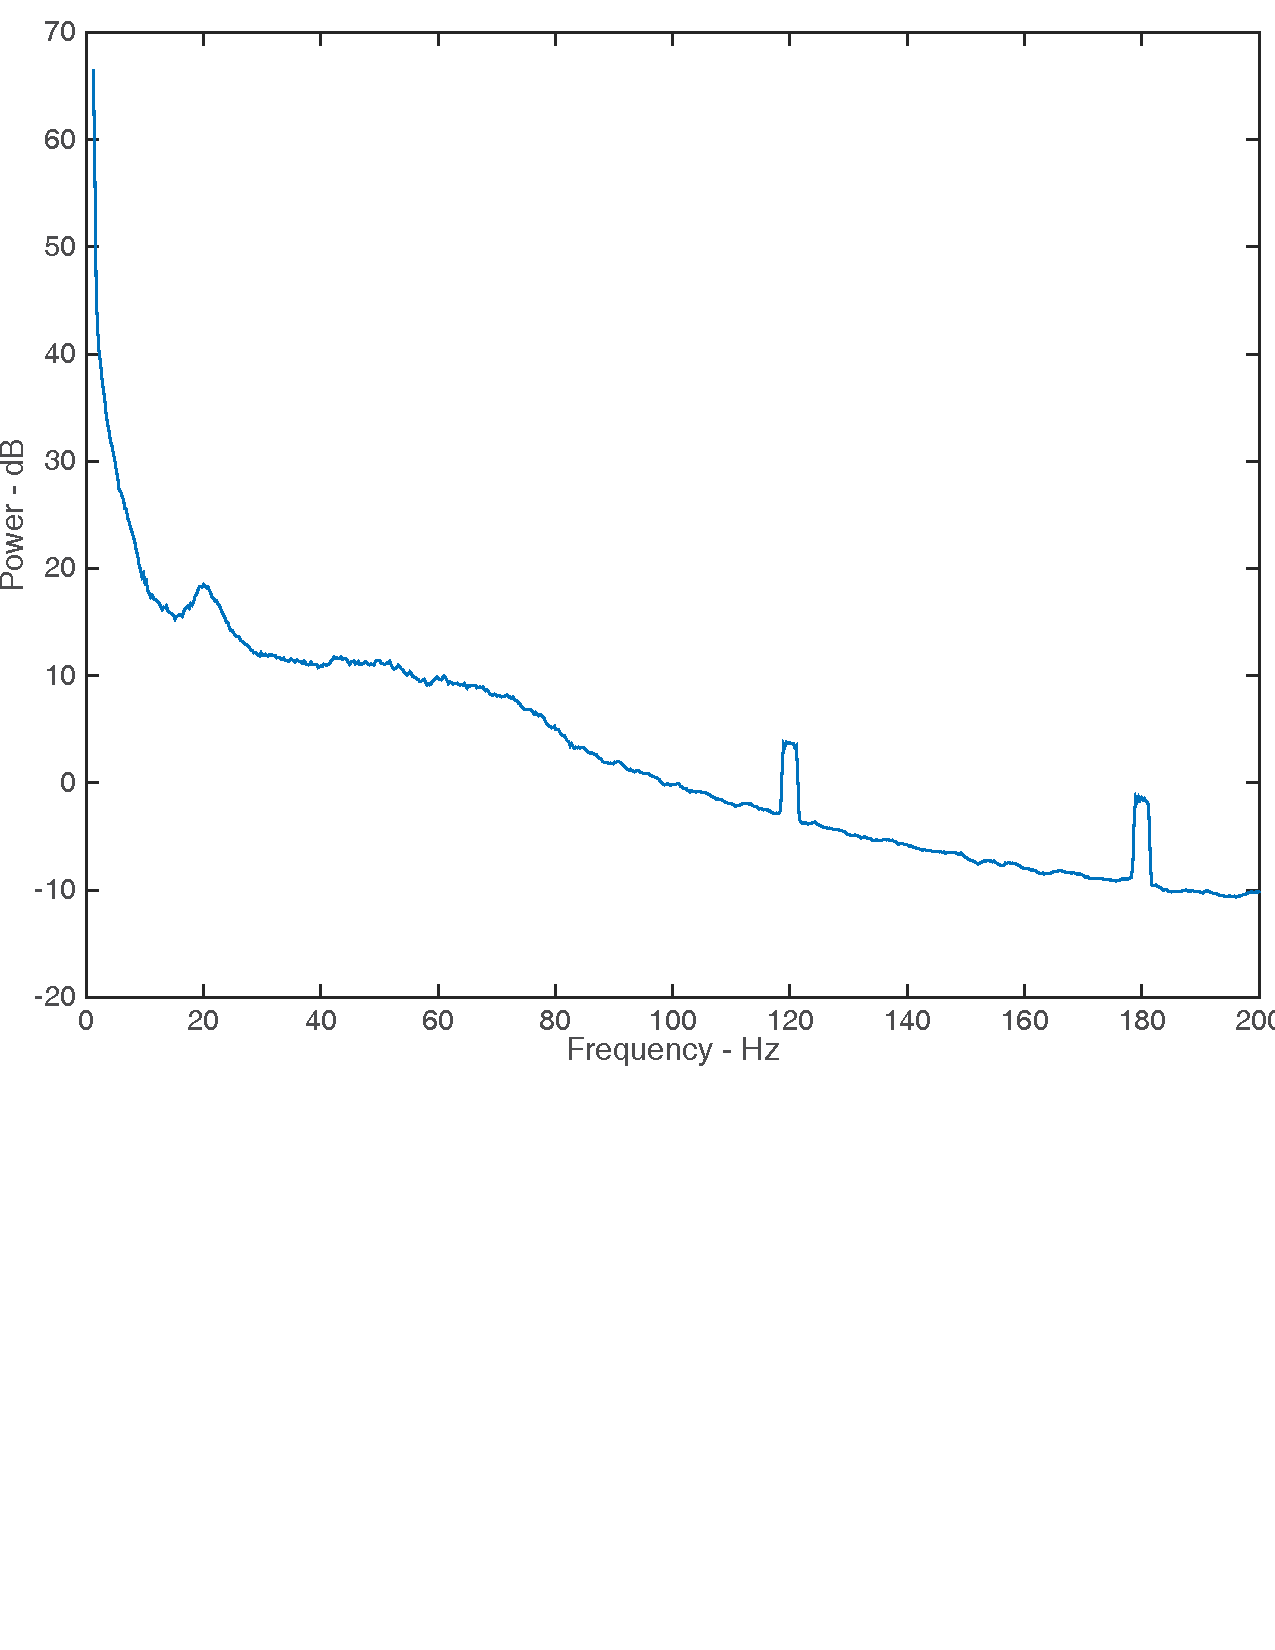
\includegraphics[width=20pc]{PSD_v1.pdf}
\caption{\label{fig:psd}Stereotypical example of power spectrum of LFP. There is a clear peak around 18-19Hz in this subject over $\beta$ range and  a small peak around 40 Hz in a low $\gamma$ range.}
\end{minipage}\hspace{2pc}
\end{figure}

First, Fig. \ref{fig:psd} shows a power spectrum of LFPs computed over $[-100, 350]$ ms of visual cue onset over 1000 consecutive cue presentations. The multi-taper method was used and the parameters used are: $[TW, K]=[3, 5]$, where $TK$ denotes the time-bandwidth product and $K$ being the number of tapers. There is a distinct peak around 18-19 Hz over the $\beta$ oscillation and a small peak around $40$Hz over the low $\gamma$ range. For the rest of the recurrence analysis, we focused on wide band oscillations: low band being $[1, 30]$ Hz to cover up to $\beta$ oscillation frequency range and the higher being $[30, 80]$ Hz to cover low $\gamma$ oscillation frequency range. 

\subsection{Temporal profiles of cluster coefficients across different bands}
The cluster coefficients for evoked responses for each channel across the two frequency bands were shown in Figs. \ref{fig:GC_low} \& \ref{fig:GC_high}. Within each frequency band, temporal variations across channels are somewhat similar. For [1,30]Hz band including the $\beta$ peak, there is a minor peak slightly before windows 150, and that particular timing is close to the highest phase locking of narrow band beta oscillaiton from this data set (18.5  $\pm$ 3 Hz , results not shown). However, other prominent features such as windows 50 and before and windows between 220-300+ are unique features that either traditional magnitude or phase analysis based on narrow band beta oscillation exhibited. 


\begin{figure}[ht!]
                             \includegraphics[scale=0.5]{fig1.pdf}
                             \caption{\label{fig:GC_low} Global clustering coefficient $C$ for the evoked response (1-30 Hz) across all channels computed with moving windows of 150 ms and 1 ms step size.The window number and the time in relation to visual cue onset are off by -100 (ms). }
\end{figure}

\begin{figure}[ht!]
                             \includegraphics[scale=0.5]{fig2.pdf}
                             \caption{\label{fig:GC_high} Global clustering coefficient $C$ for the evoked response (30-80 Hz) across all channels computed with moving windows of 150 ms and 1 ms step size.}
\end{figure}
 Compared to the lower frequency band, low $\gamma$ band apparently show more heterogeneous temporal variations across channels and timing at which high $C$ values are attained are almost opposite (except for the first tens of windows). Furthermore the timing at which local maxima are attained between windows 100 to 200 vary significantly from 0 to 2, especially compared to [1,30]Hz band where the peak C timing in that window roughly corresponds to the highest phase locking. 
 
 \begin{figure}[ht!]
                             \includegraphics[scale=0.35]{low_vs_high_C_variation.pdf}
                             \caption{\label{fig:GC_comp} Variations of global clustering coefficients across channels for the two different bands. Each plot shows mean $\pm$ std computed over all the channels used for the analysis. Top for low frequency range, [1,30]Hz. Bottom for high frequency (or low $\gamma$ range [30,80]Hz. }
\end{figure}
Then, we looked at the temporal variations of the C values across channels in Fig. \ref{fig:GC_comp}. The standard deviation at any given time point for both frequency bands are somewhat compatible, but the mean trends show almost opposite behavior. Furthermore, probably due to phase locking over the $\beta$ range, the temporal trajectory of C quickly changes over windows 100 to 200. Therefore, the recurrence network analysis, even at the level of evoked potentials exhibit much richer response patterns than simple narrow band phase locking or wide band amplitude trajectories. 

  \subsection{Optimal delay}
  
  Fig. \ref{fig:OptDelay} shows the auto-mutual information for an exemplary channel. It can be seen from Fig. \ref{fig:OptDelay}  that the first local minimum of the auto-mutual information occurs at a lag of 5. Similar behavior was seen for most of signals from other channels. 
\begin{figure}[ht!]
                             \includegraphics[scale=0.5]{fig3.pdf}
                             \caption{\label{fig:OptDelay} Optimal delay $\tau$ using auto-mutual information for an exemplary channel. The red line denotes the first local minimum.}
\end{figure}
 
 \subsection{Embedding dimension}

Fig. \ref{fig:min_emb}  shown the plot of FNN statistic with respect to the embedding dimension for an exemplary signal. Already at an embedding dimension of 3, the value of FNN statistic drops to 0.04. Given the amount of data in each window (150 sample points), the choice of m = 3 seems feasible. Going for larger values of m like 5 or 6 might greatly reduce the amount of points needed to estimate the network characteristics. For the sake of consistency, based of these observations, we set optimal delay $\tau = 5$ and embedding dimension $m = 3$  to reconstruct the phase space vector from all the signals.

\begin{figure}[ht!]
                             \includegraphics[scale=0.5]{fig4.pdf}
                             \caption{\label{fig:min_emb} Minimum embedding $m$ using the FNN method for an exemplary channel. At $m=3$, the FNN statistic is already below 0.05}
\end{figure}


\section{Discussions}
\label{sec:discussions}
Based on our previous work \cite{MattNER2013}, we had shown that the relative power of $\beta$ oscillation and $\gamma$ oscillation changed around the movement onset and that there were effectively three states based on the ratios of $\beta$ and $\gamma$ powers averaged over all the channels from our MI array. In our current work, we applied recurrence network analysis to wide band signals containing $\beta$ range and the low $\gamma$ range. Although the computations are more involved, our analysis capture richer
 dynamics of  wide band signals and clear control of the underlying network dynamics during the task
 based only on evoked responses in LFPs. 

 In our current study, we only looked at temporal dynamics of recurrence network analysis,  but we would like to extend the method to characterize spatiotemporal dynamics of cortical signals as we used phase based method to characterize wave propagation of narrow-band filtered signals \cite{doug2006betawave}. Particularly, the current method can be very attractive to study wide(r) band signals such as low and high $\gamma$ oscillations for which phase calculation can be non-trivial. 







\section{Acknowledgement}
The authors would like to thank H. Watanabe in Department of Developmental Physiology at National Institute for Physiological Sciences (NIPS) at Okazaki, Japan for usual discussions,  and members of Hatsopoulos laboratory at University of Chicago for surgery,  training, and data collection from monkeys and discussions. 

\bibliographystyle{IEEEbib}
\bibliography{refs}
\end{document}